\documentclass[openany,12pt,UTF8]{article}
\usepackage[a4paper,margin=2.5cm]{geometry}
\usepackage{amsmath}                                    % 排版数学公式

% 使equation计数器也依赖于section计数器
\numberwithin{equation}{section}

% 使table计数器也依赖于section计数器
\numberwithin{table}{section}

% 使figure计数器也依赖于section计数器
\numberwithin{figure}{section}

\usepackage{latexsym}
\usepackage{amsfonts}                                   %数学符号字体库宏包套件,它包含有:amsfonts、amssymb、eufrak 和 eucal 四个宏包。
\usepackage{amssymb}                                    % 定义AMS的数学符号命令
\usepackage{mathrsfs}                                   % 数学RSFS书写字体
\usepackage{bm}                                         % 数学黑体
\usepackage{graphicx}                                   % 支持插图,图形宏包graphics的扩展宏包
\usepackage{color,xcolor}                               % 支持彩色
\usepackage{amscd}
\usepackage[linesnumbered,ruled,vlined]{algorithm2e}
\usepackage{diagbox}
\usepackage{minted}
\usepackage{titlesec}                                   %设置章节格式
\usepackage{tcolorbox}

% 设置 paragraph 为只有一级编号(从1开始)
\renewcommand{\theparagraph}{\arabic{paragraph}} % 只显示一级编号
\makeatletter
\@addtoreset{paragraph}{section} % 每节开始时重置 paragraph 计数器
\makeatother

%%文本框设置
\newcommand{\tbox}[1]{
  \begin{center}
    \begin{tcolorbox}[colback=gray!10,%gray background
        colframe=black,% black frame colour
        width=14cm,% Use 8cm total width,
        arc=1mm, auto outer arc,
        boxrule=0.5pt,
      ]
      {#1}
    \end{tcolorbox}
  \end{center}
}

% 设置 paragraph 为 block 风格,自动换行
\titleformat{\paragraph}[block]
  {\normalfont\normalsize\bfseries}{\theparagraph.}{0.5em}{}

% 设置标题后换行(after-sep 设为 \newline)
\titlespacing*{\paragraph}{0pt}{3.25ex plus 1ex minus .2ex}{0pt}
  
\usepackage{enumerate}                                 	%更改enumerate环境格式
\usepackage{hyperref}

%改变超链接颜色
\hypersetup{
    colorlinks=true,
    linkcolor=blue,
    filecolor=blue,      
    urlcolor=blue,
    citecolor=cyan,
}

\usepackage{subcaption}
\usepackage{minipage-marginpar}
\usepackage{float}%提供float浮动环境
\usepackage{booktabs}%提供命令\toprule、\midrule、\bottomrule
\usepackage{listings}
\usepackage{xcolor}
\usepackage{tabularx}
\usepackage{multirow}
\usepackage[perpage]{footmisc}

% 自定义命令,用于角标引用文献和交叉引用
\newcommand{\scite}[1]{\textsuperscript{\cite{#1}}}
\newcommand{\sref}[1]{\textsuperscript{\ref{#1}}}
\newcommand{\bs}[1]{\boldsymbol{#1}}
\newcommand{\romannumber}[1]{\uppercase\expandafter{\romannumeral#1}}
\newcommand{\alert}[1]{\textcolor{red}{#1}}

% 设置标题层级和目录层级
\setcounter{tocdepth}{3}
\setcounter{secnumdepth}{4}

% ----------------------------
% 代码显示相关宏包
% ----------------------------
\usepackage{listings}     % 代码高亮

% ----------------------------
% 设置代码样式
% ----------------------------
\definecolor{codegray}{rgb}{0.5,0.5,0.5}
\definecolor{backcolor}{rgb}{0.95,0.95,0.95}
\definecolor{codeblue}{rgb}{0.2,0.2,0.6}
\definecolor{keywordcolor}{rgb}{0.1,0.1,0.6}
\definecolor{stringcolor}{rgb}{0.58,0,0.1}

\lstdefinestyle{pythonstyle}{
    backgroundcolor=\color{backcolor},   
    commentstyle=\color{codegray}\itshape,
    keywordstyle=\color{keywordcolor}\bfseries,
    stringstyle=\color{stringcolor},
    numberstyle=\tiny\color{gray},
    basicstyle=\ttfamily\footnotesize,
    breaklines=true,                     
    captionpos=b,                        
    keepspaces=true,
    numbers=left,                        
    numbersep=5pt,                       
    showspaces=false,                    
    showstringspaces=false,
    showtabs=false,                      
    tabsize=4,
    language=Python
}

% 设置默认样式
\lstset{style=pythonstyle}

\usepackage{rotating}
\title{Simulation Practice Report for Statistics of Flight Experiment}
\author{Ouyang Jiahong}
\date{\today}
\begin{document}
\maketitle
\newpage
\tableofcontents
\newpage

\section{Introduction of the simulation task}
In this project, we investigate two classical parameter estimation techniques—Batch Least Squares (BLS) and Recursive Least Squares (RLS)—to estimate the bias and scale factor of gyroscope sensors. The BLS method solves a global least squares optimization problem over all available data, yielding a static estimate of the parameters. In contrast, the RLS algorithm updates the parameter estimates incrementally with each new observation, making it suitable for real-time or adaptive scenarios.

Both methods consider the impact of the Earth's rotation on the gyroscope's output by incorporating a correction term based on latitude. Experiments are conducted using a dataset consisting of 50 groups of measurements, each containing 500 samples from a 7-channel gyroscope. The estimation results from BLS and RLS—with different initialization strategies—are compared in terms of residual errors and convergence behavior.

\subsection{Background}
\subsubsection{Gyroscope Measurement Model}
\begin{equation}
    \label{equation:Gyroscope Measurement Model}
    \omega_{G} = \underbrace{E_{\omega 0}}_{\text{Bias}} + \underbrace{E_{\omega 1}}_{\text{Factor}} \cdot (\omega + \text{Vel}_{ver}) + \varepsilon_{G}
\end{equation}

\subsubsection{Input Data}
\paragraph{Angular Velocity Input}\
\begin{equation}
    \omega = [60\ 40\ 50\ 80\ 33\ 24\ 17]^{\text{T}} \ (\circ/\text{s})
\end{equation}

\paragraph{Measurement Noise}\
\begin{equation}
    \varepsilon_{G} \sim N(0,\ 1 \times 10^{-8})
\end{equation}
This represents a Gaussian white noise with zero mean and variance of $1 \times 10^{-8}$.

\subsubsection{Latitude and Vertical Angular Velocity}
\paragraph{Geographic Latitude (PhiN)}\
\begin{equation}
    \text{PhiN} = 28.209167\ ^\circ
\end{equation}

\paragraph{Vertical Angular Velocity (Considering Earth's Rotation)}\
\begin{equation}
    \text{Vel}_{ver} = 7.292 \times 10^{-5} \times \text{r2d} \times \sin(\text{PhiN} \times \text{d2r})
\end{equation}
Where:
\begin{itemize}
    \item \texttt{r2d} denotes conversion from radians to degrees (i.e., $180/\pi$)
    \item \texttt{d2r} denotes conversion from degrees to radians (i.e., $\pi/180$)
\end{itemize}

\paragraph{Sampling Step}\

0.01 seconds

\subsection{Assignment}
\begin{enumerate}
    \item Please estimate the bias and factor of a gyro using batch LS and RLS, and compare the estimation solutions.
    \item When the batch LS is employed, please estimate the variance of measurement noise.
    \item When the RLS is employed, please answer the following questions by simulations:
          \begin{itemize}
              \item How the estimation error curve will vary when the initial parameter is set as the BLS solution and when the initial parameter is randomly set?
              \item How the estimation error curve of parameter is affected by the initial conditions?
          \end{itemize}
\end{enumerate}

\subsection{Description of Provided Data Formats}
\subsubsection{GyroMeasData\_X.mat}
In \texttt{GyroMeasData\_X.mat}, there is a 500×7 double-precision data matrix. Each row of data (1×7) represents one observation of $\omega$. X represents the experiment number, ranging from 0 to 100. We will use the 500 observations from X experiments to estimate Bias and Factor, as shown in \autoref{equation:Gyroscope Measurement Model}.

\subsubsection{GyroBias.mat}
In \texttt{GyroBias.mat}, there is a 1×100 double-precision data array. Each element represents the true value of Bias for one experiment. For example, GyroBias[1] represents the Bias true value for X=1, which corresponds to the experiment stored in GyroMeasData\_1.mat. After estimating \texttt{estimate\_bias} using data from \texttt{GyroMeasData\_X.mat}, it should be compared with the true values.

\subsubsection{GyroFactor.mat}
In \texttt{GyroFactor.mat}, there is a 1×100 double-precision data array. Each element represents the true value of Factor for one experiment. For example, GyroFactor[1] represents the Factor true value for X=1, corresponding to the experiment in GyroMeasData\_1.mat. After calculating \texttt{estimate\_factor} using data from \texttt{GyroMeasData\_X.mat}, it should be compared with the true values.

\section{Introduction of the algorithm investigated}
In this study, we investigate and compare two classical parameter estimation techniques applied to the calibration of gyroscope measurements: \textbf{Batch Least Squares (BLS)} and \textbf{Recursive Least Squares (RLS)}. The target is to jointly estimate the bias and scale factor (denoted as "factor") of a multi-channel gyroscope, based on synthetic measurement data generated from known ground truth parameters and corrupted with realistic noise.

The underlying measurement model assumes that the observed gyroscope readings $\omega_G$ are linearly related to the true angular rate input $\omega$ via the relation:
$$
\omega_G = \text{bias} + \text{factor} \cdot (\omega + \omega_E)
$$

where $\omega_E$ denotes the effect of Earth's rotation in the local vertical direction, accounted for using the latitude of the test site. This correction is computed as:
$$
\omega_E = 7.292 \times 10^{-5} \cdot \frac{180}{\pi} \cdot \sin(\phi)
$$
with $\phi$ representing the latitude (here, $\phi = 28.209167^\circ$).

The \textbf{Batch Least Squares (BLS)} method estimates the bias and factor parameters by stacking all measurement equations into a single linear system and solving it via the normal equations. It is a non-iterative method that leverages all available data at once to obtain a point estimate.

In contrast, the \textbf{Recursive Least Squares (RLS)} method updates the parameter estimates iteratively with each new observation. It is particularly useful in online or real-time estimation scenarios, where measurements arrive sequentially. The RLS algorithm uses a gain matrix and an evolving estimate covariance matrix to balance prior knowledge with new observations. In our implementation, we initialize RLS with either a random guess perturbed by a small factor, or with the result from the BLS estimate, to examine the sensitivity of convergence.

Experimental evaluation is conducted on 50 synthetic datasets, each containing 500 measurements across 7 axes. The effectiveness of both algorithms is assessed in terms of estimation accuracy (residuals compared to ground truth) and convergence speed. Visualization of residuals and convergence behavior provides insights into estimator performance under different initialization conditions.

\section{Results and Analysis}

\subsection{Results of Simulations}

\subsubsection{Residuals of Bias Estimation}
\autoref{figure:Residuals of Bias Estimation} shows the bias estimation residuals across 50 experiments. All methods—BLS (blue circles), RLS with random initialization (red lines), and RLS with BLS initialization (green dashed lines)—exhibit residuals within $10^{-6}$. A black dashed zero-line serves as reference.

\begin{figure}[h]\centering
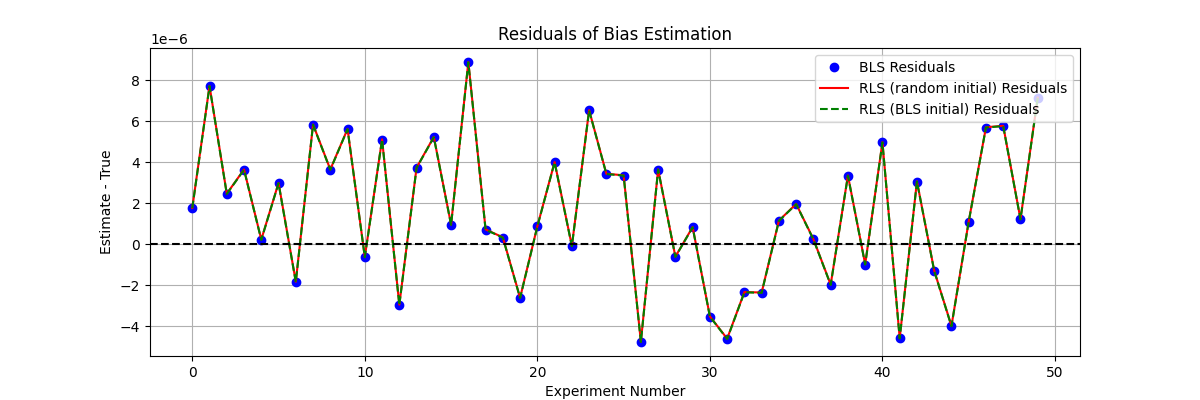
\includegraphics[width=\columnwidth]{figures/Residuals of Bias Estimation.png}
\caption{Residuals of Bias Estimation}
\label{figure:Residuals of Bias Estimation}
\end{figure}

\subsubsection{Residuals of Factor Estimation}
\autoref{figure:Residuals of Factor Estimation} presents the factor estimation residuals. All methods maintain residuals within $10^{-7}$, showing similarly high accuracy. Series labels and formatting are consistent with the previous figure.

\begin{figure}[h]\centering
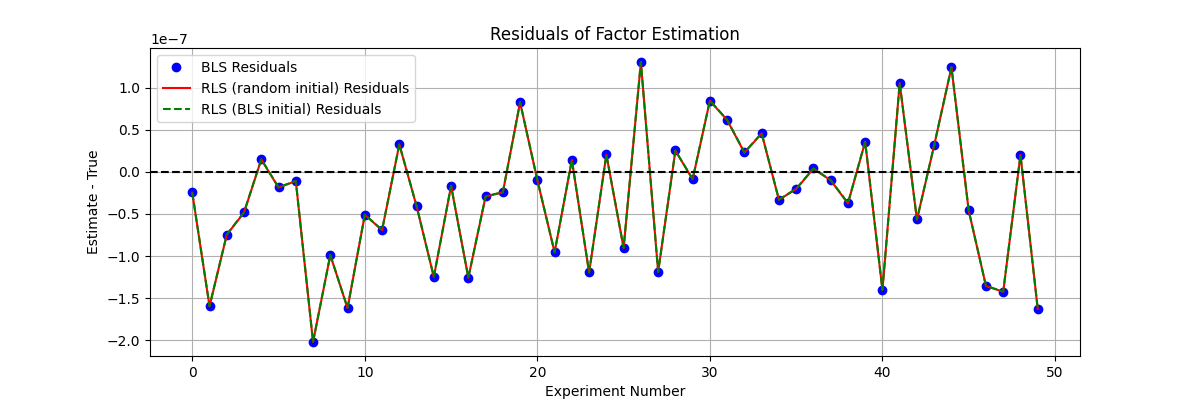
\includegraphics[width=\columnwidth]{figures/Residuals of Factor Estimation.png}
\caption{Residuals of Factor Estimation}
\label{figure:Residuals of Factor Estimation}
\end{figure}

\subsubsection{Bias and Factor Estimation of Exp 1}
\autoref{figure:Bias and Factor Estimation of Exp 1} illustrates convergence behavior in a single experiment. Initializing RLS with BLS slightly improves convergence speed, though the effect is limited. True values are shown as black dashed lines.

\begin{figure}[h]\centering
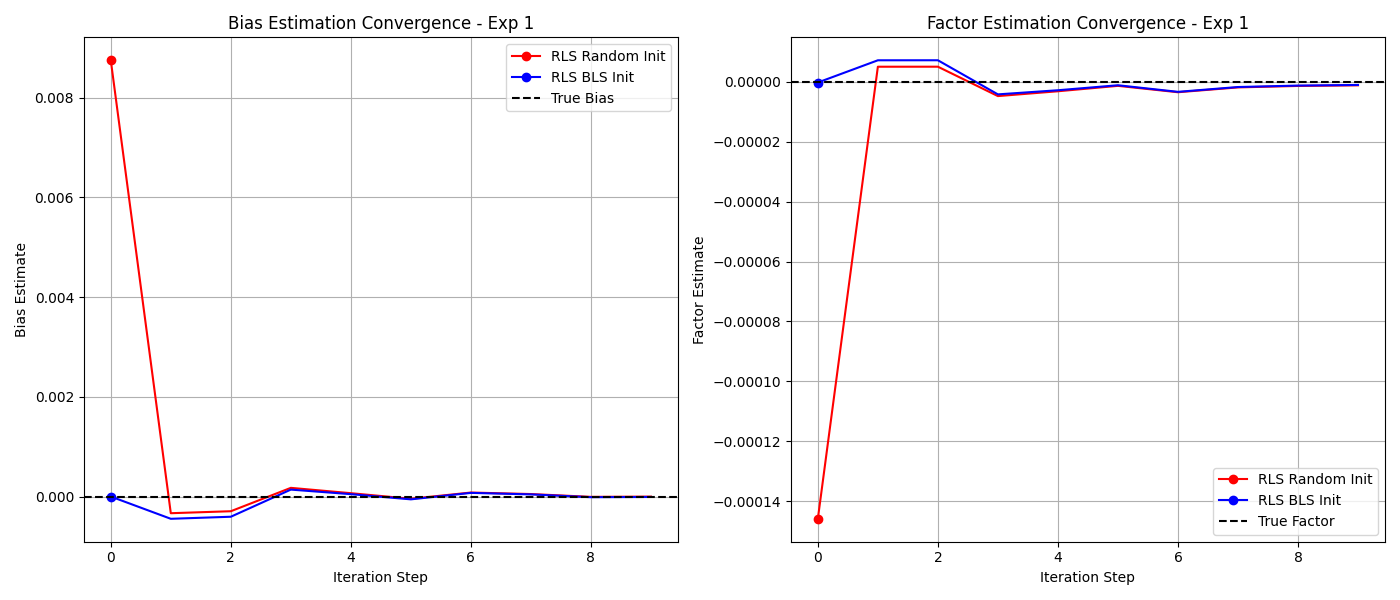
\includegraphics[width=\columnwidth]{figures/Bias and Factor Estimation of Exp 1.png}
\caption{Bias and Factor Estimation of Exp 1}
\label{figure:Bias and Factor Estimation of Exp 1}
\end{figure}

\subsubsection{Bias and Factor Estimation of All Exp}
\autoref{figure:Bias and Factor Estimation of All Exp} summarizes convergence trends across all experiments. Both RLS variants ultimately approach the true values. RLS with BLS initialization converges slightly faster and more smoothly.

\begin{figure}[h]\centering
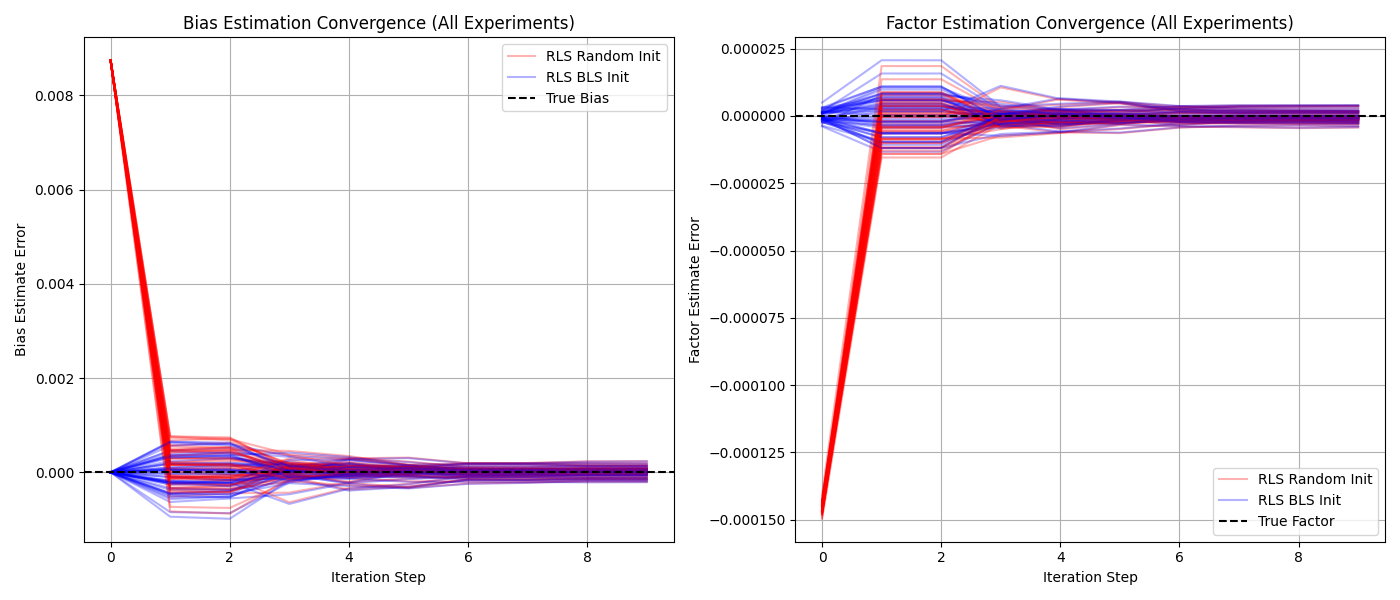
\includegraphics[width=\columnwidth]{figures/Bias and Factor Estimation of All Exp.png}
\caption{Bias and Factor Estimation of All Exp}
\label{figure:Bias and Factor Estimation of All Exp}
\end{figure}

\subsection{Analysis}
From the results above, both BLS and RLS yield highly accurate estimations, with residuals consistently within the magnitude of $10^{-6}$ for bias and $10^{-7}$ for factor across 50 experiments. This suggests that the problem is well-conditioned and the measurement noise is sufficiently small, enabling robust estimation by both methods.

Second, the RLS method initialized with BLS results shows slightly faster convergence compared to RLS with random initialization. As shown in \autoref{figure:Bias and Factor Estimation of Exp 1} and \autoref{figure:Bias and Factor Estimation of All Exp}, the improvement is marginal in these experiments. In theory, RLS with BLS initialization should achieve smoother and more stable convergence, as a good prior helps accelerate learning and reduces transient fluctuations.

Third, there is negligible difference in the final estimation accuracy between the two RLS variants. After sufficient iterations, both converge to results nearly identical to those from BLS. This confirms the theoretical expectation that RLS asymptotically approaches BLS given enough data, assuming the measurement model remains linear and the noise characteristics are stationary.

In conclusion, both BLS and RLS are effective in this scenario. While BLS provides a reliable offline solution, RLS offers the added benefit of online adaptability. Initializing RLS with BLS results can marginally improve convergence speed, which may be advantageous in real-time applications.

\section*{Appendix: Python Code}

\subsection*{A.1 Core Algorithm Implementation}

\lstinputlisting[language=Python,caption={Main Estimation Algorithm Implementation}]{../fun.py}

\subsection*{A.2 Data Processing Module}

\lstinputlisting[language=Python,caption={Data Processing Module}]{../data.py}

\subsection*{A.3 Function Main Entry \& Visualization Module}

\lstinputlisting[language=Python,caption={Function Main Entry \& Visualization Module}]{../main.py}
\end{document}